% !TEX root = ../0-main-LN.tex

\begin{center}
	{\Large\bf 微积分学前自测}
	
	{\it 注:以下练习均与本课程后续内容相关,请务必自行学习掌握}
\end{center}
\begin{enumerate}
  \item 请在图上标出常用的三角函数值:
  $\sin\theta,\;\cos\theta,\;\tan\theta,\;
  \sec\theta,\;\csc\theta.$
  \ps{$\sec\theta=\df1{\cos\theta}$,\\ $\csc\theta=\df1{\sin\theta}$}
  \begin{figure}[!htb]
  	\centering
  	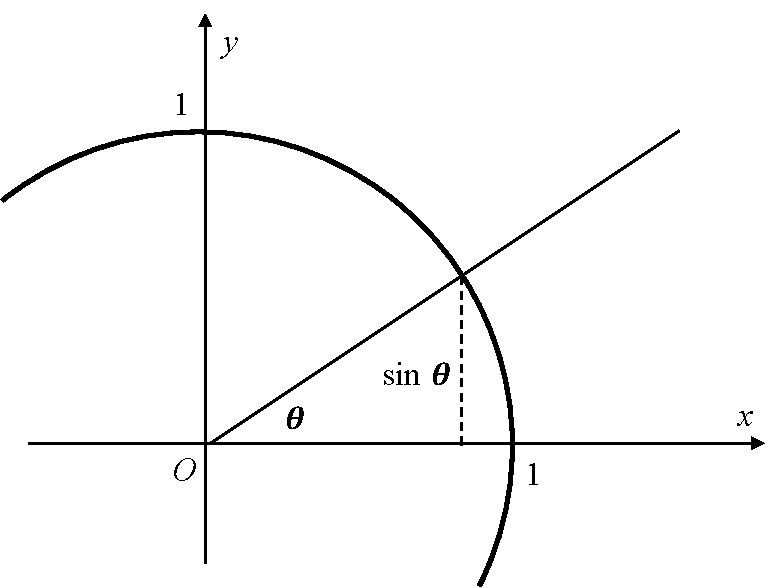
\includegraphics[width=0.6\textwidth]{./Images/ch00/selfTest/triFuncs.pdf}
  \end{figure}
  \item 三角函数的反函数统称为{\kaishu 反三角函数},因为三角函数都是周期函数,
  在整个定义域上不具有统一的单调性,其反函数只能以其某个周期内的一部分为基础来讨论。
  例如:对于正弦函数$y=\sin x$,我们选择其在$[-\pi/2,\pi/2]$上的一段,
  在该区间上$y=\sin x$是严格单调递增的,其反函数记为$y=\arcsin x$
  \ps{相应地反余弦记为$\arccos x$,反正切记为$\arctan x$}。
  $y=\arcsin x$的定义域是$[-1,1]$,值域为$[-\pi/2,\pi/2]$,其图像与
  $y=\sin x$在$[-\pi/2,\pi/2]$区间上的图像关于$y=x$对称。
  从这个例子出发,我们可以很容易地理解讨论反三角函数的基本原则:
  {\kaishu(1)选择三角函数的一个单调区间;(2)所选择的区间
  应该靠近原点,具体来说:要么原点为所选区间的中心,要么为其左端点(也即
  优先考虑正半轴上的区间)}。基于对以上叙述的理解,请分别给出
  $\arccos x$、$\arctan x$的定义域和值域,并试着画出其图像。
  \item 描绘下列函数的图形:
  \begin{center}
    $\sin(\arcsin x),\quad \arcsin(\sin x),\quad
    \tan(\arctan x),\quad \arctan(\tan x)$
  \end{center}
  \item 化简如下表达式
  \begin{enumerate}[(1)]
    \item $\cos(\arcsin x)$
    \item $\sin(\arctan x)$
  \end{enumerate}
  \item 证明:
  $$\df{\pi}4=3\arctan\df14+\arctan\df5{99}$$
  \item 证明:
  $$3\arccos x-\arccos(3x-4x^3)=\pi,\;\left(|x|\leq\df12\right)$$
  \item 平面上任一点的位置可以既可以用直角坐标$(x,y)$表示,也可以用极坐标$(\rho,\theta)$
  表示,前者可用后者表示如下
  $$x(\rho,\theta)=\rho\cos\theta,\quad y(\rho,\theta)=\rho\sin\theta,$$
  反之,后者用前者应表示为(假设:$\rho\geq 0,\theta\in[0,2\pi]$)
  $$\rho(x,y)=\underline{\hspace{5cm}},\quad
  \theta(x,y)=\underline{\hspace{5cm}}.$$
  \item 比较以下函数值的大小,简述理由
  \begin{enumerate}[(1)]
    \item $x,\quad e^x-1,\quad \ln(x+1)$\quad$(x>0)$
    \item $\sin x,\quad \tan x, \quad \sec x, \quad x$ \quad $(x\in(0,\pi))$
  \end{enumerate}
  \item 证明函数$y=x+\sin x$在定义域内严格单调递增。({\it 注:函数$y=f(x)$严格单调
  递增,当且仅当对任意$x_1<x_2$,总有$f(x_1)<f(x_2)$})
  \item 证明:任何一个定义在对称区间上的函数均可写成一个奇函数和一个
  偶函数的和;并由此写出$e^x$是由怎样的奇函数和偶函数相加而成。
  \item 写出下列集合之间的一一映射
  \begin{enumerate}[(1)]
    \item $(-1,1)\mapsto\mathbb{R}$
    \ps{$\mathbb{R}=(-\infty,+\infty)$}
    \item $(0,+\infty)\mapsto\mathbb{R}$
    \item $\{(x,y)\in\mathbb{R}^2|x^2+y^2<1\}\mapsto\mathbb{R}^2$
    \ps{\it $\mathbb{R}^2$表示全平面}
    \item 整数集$\mapsto$正整数集
  \end{enumerate}
  \item Fibnacci数列定义如下:$a_0=1$,$a_1=1$,
  $$a_{n+2}=a_{n+1}+a_{n},\quad n=1,2,\ldots,$$
  \begin{enumerate}[(1)]
    \item 请推导$\{a_n\}$的通项表达式;
    \item 设$p,q\in\mathbb{R}$,将前述递推式改为:
    $$a_{n+2}=p\cdot a_{n+1}+q\cdot a_{n},\quad n=1,2,\ldots,$$
    试讨论$\{a_n\}$通项表达式有何变化。
  \end{enumerate}
  \item 写出不少于五位你听说过的数学家的名字(最好用英文),简述他们的事迹。
  \item 公理(Axiom)、假设(Assumption)、定理(Theorem)、定律(Law)有何异同?
  \item 取整函数$[x]$的定义为{\it 不大于$x$的最大整数},请利用取整函数给出以下曲线的方程:
  \begin{center}
	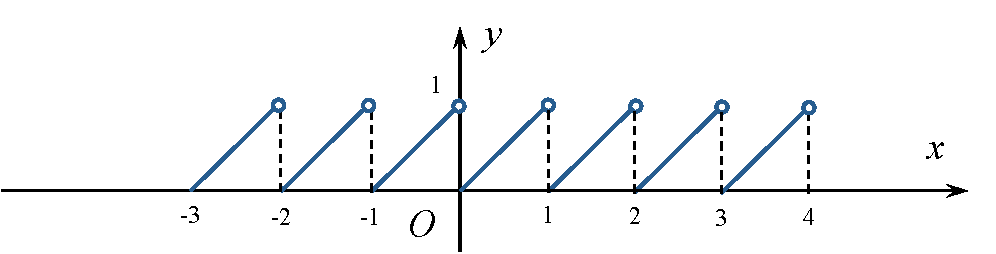
\includegraphics[width=0.8\textwidth]{./images/ch00/selfTest/ST-Func1.pdf}\\
	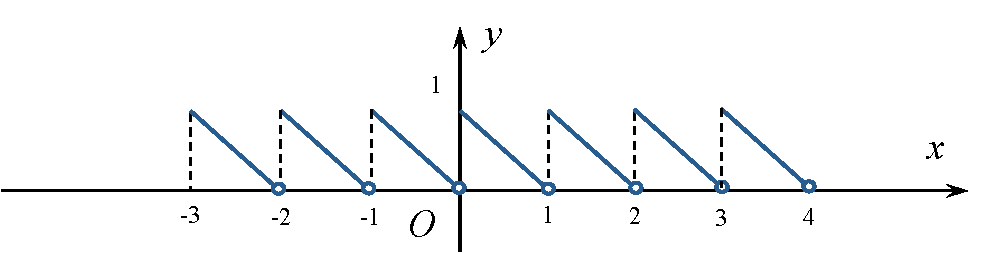
\includegraphics[width=0.8\textwidth]{./images/ch00/selfTest/ST-Func2.pdf}\\
	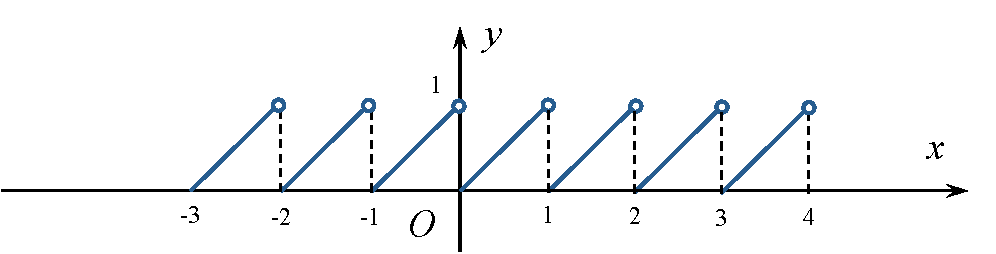
\includegraphics[width=0.8\textwidth]{./images/ch00/selfTest/ST-Func1.pdf}
  \end{center}
  \item 设$a\in\mathbb{R}$,且对任意$x\in\mathbb{R}$,有
  $f(2a-x)=f(x)$,
  请问$y=f(x)$的图像具有怎样的几何性质?若上式改为$f(2a-x)=-f(x)$,对应几何性质有何改变?
  \item 设$a\in\mathbb{R}$,且对任意$x\in\mathbb{R}$,有
  $f(a-x)=g(x)$,请问$y=f(x)$和$y=g(x)$的图像有何关系?
  \item 若对任意$x_1,x_2$,总有
  $[f(x_1)-f(x_2)](x_1-x_2)\leq 0$,
  由此可知函数$y=f(x)$具有何种性质?
  \item 给定集合$A\subset\mathbb{R}$,若$A$有界
  \ps{集合$A$有界,是指存在某个数$M$,对任意$x\in A$,总有$|x|\leq M$},是否必有最大和最小值?
  是否必有{\it 上确界}(即最小的上界)和{\it 下确界}(即最大的下界)?
  若$A$无界,是否必为无穷集合(即集合中的元素个数不是有限的)?
\end{enumerate}